\documentclass{article}

\usepackage{microtype}
\usepackage{graphicx}
\usepackage{subcaption}
\usepackage{booktabs}
\usepackage{hyperref}
\usepackage{xcolor}
\usepackage{multirow}

\newcommand{\theHalgorithm}{\arabic{algorithm}}

\usepackage{icml2026}

\usepackage{amsmath}
\usepackage{amssymb}
\usepackage{mathtools}
\usepackage{amsthm}

\usepackage[capitalize,noabbrev]{cleveref}
 \newcommand{\michael}[1]{\textcolor{blue}{\small [#1] - michael}}
  \newcommand{\matt}[1]{\textcolor{red}{\small [#1] -matt}}

\icmltitlerunning{VFUSE: Virulent Feature Understanding with Sparse autoEncoders}

\begin{document}

\twocolumn[
  \icmltitle{VFUSE: Virulent Feature Understanding with Sparse autoEncoders
}

  \icmlsetsymbol{equal}{*}

  \begin{icmlauthorlist}
    \icmlauthor{Anonymous}{anon}
  \end{icmlauthorlist}

  \icmlaffiliation{anon}{Anonymous Submission}

  \icmlcorrespondingauthor{Anonymous}{anon@anon.org}

  \icmlkeywords{sparse autoencoders, mechanistic interpretability, protein diffusion, biosecurity, RFdiffusion}

  \vskip 0.3in
]

\printAffiliationsAndNotice{}

\begin{abstract}
Generative models have shown remarkable progress in a variety of domains such as protein design, but such power enables the opaque generation of hazardous proteins. In this work, we introduce VFUSE (Virulent Feature Understanding with Sparse autoEncoders), a mechanistic interpretability approach that trains SAEs on diffusion-transformer activations to audit protein models for hazard-aware features. We apply VFUSE to RoseTTAFold3 and RFDiffusion3, popular open-weight models for protein folding and synthesis. We find that at block 12 of RFD3, probes trained on SAE-encoded features outperform raw-activation probes by $+0.054$ AUROC under homology-clustered evaluation. Furthermore, we identify individual SAE features that fire preferentially on hazardous designs, reaching up to AUROC $0.84$ ($q < 10^{-13}$). To our knowledge this is the first SAE trained on an all-atom diffusion model and the first feature-level virulence audit of a protein design model, paving the way towards safe and interpretable protein design.\footnote{Code available at \url{https://anonymous.4open.science/r/vfuse-B834/README.md}}

\end{abstract}


\section{Introduction}
\label{sec:intro}

Protein diffusion models can now design binders, enzymes, and oligomers that are validated to fold in the wet lab \cite{watson2023rfdiffusion,krishna2024rfaa,butcher2025rfdiffusion3,woolfson2021brief}. This capability is dual-use: given a hazardous template such as a neurotoxin active site, a diffusion model can scaffold new proteins around it. Existing biosecurity screens rely on sequence homology or sequence-level classifiers \cite{garg2008virulentpred,singh2024vfpred,sun2024dtvf,chen2025virulenthunter}. They flag a sequence after the fact but cannot explain which structural features triggered the flag, and they cannot intervene during sampling.

Mechanistic interpretability has made substantial progress in understanding language models \cite{bricken2023monosemanticity,cunningham2024sparse,templeton2024scaling} and, more recently, vision models \cite{joseph2025prisma,simonyan2014deep,Ben_Melech_Stan_2024_CVPR}. Sparse autoencoders (SAEs) decompose dense latent activations into sparse, approximately monosemantic directions, and have been applied to protein language models \cite{simon2025interplm,adams2025mechanistic,parsan2025interpretable}. All-atom diffusion models have not, however, been similarly probed.

Applying VFUSE to RFdiffusion3 (RFD3) and RoseTTAFold3 (RF3), we find that at block 12 of RFD3, SAE-encoded representations outperform raw activations as probe inputs, and that individual VFUSE-discovered features fire selectively on hazardous designs with per-residue localization (See \Cref{fig:features}). We release SAE checkpoints at three depths in RFD3 and two in RF3, together with a catalogue of hazard-associated features.

\begin{figure*}[tb]
\centering
\begin{subfigure}[t]{0.245\linewidth}
  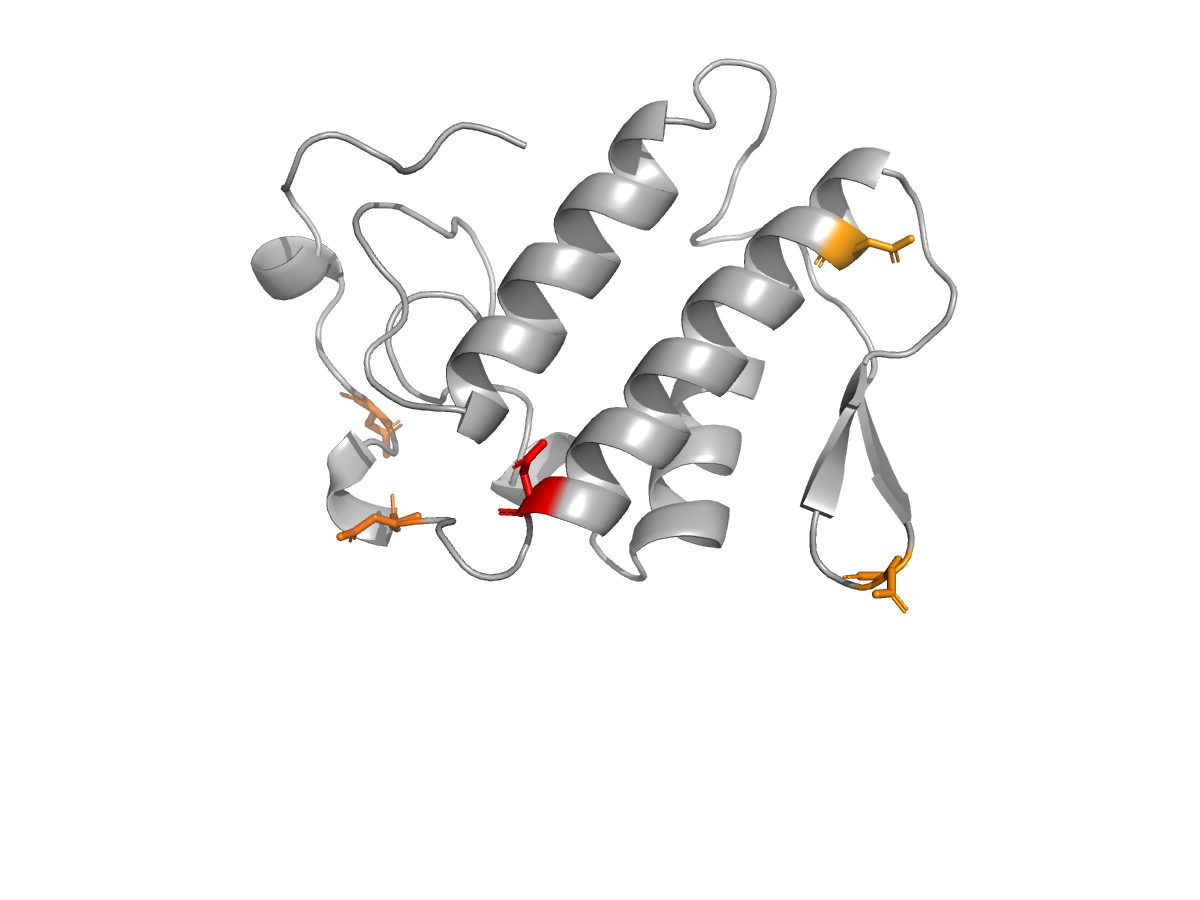
\includegraphics[width=\linewidth]{figures/feat639_P00626.png}
  \caption{\textbf{Feature 639} (AUROC 0.819)\\Ammodytoxin A (P00626)\\Viper neurotoxin}
\end{subfigure}\hfill
\begin{subfigure}[t]{0.245\linewidth}
  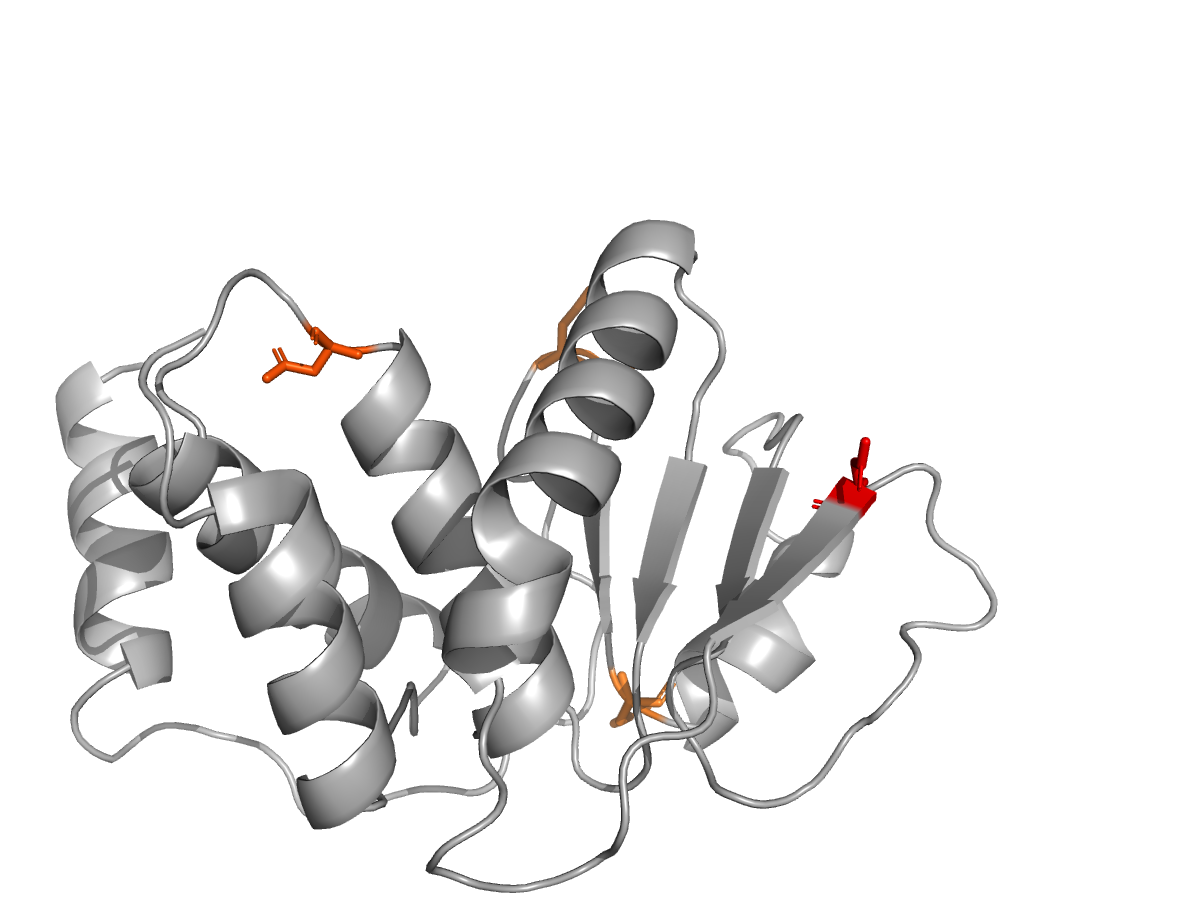
\includegraphics[width=\linewidth]{figures/feat060_MPXV.png}
  \caption{\textbf{Feature 60} (AUROC 0.813)\\OPG106 (A0A7H0DN78)\\Monkeypox immune evasion}
\end{subfigure}\hfill
\begin{subfigure}[t]{0.245\linewidth}
  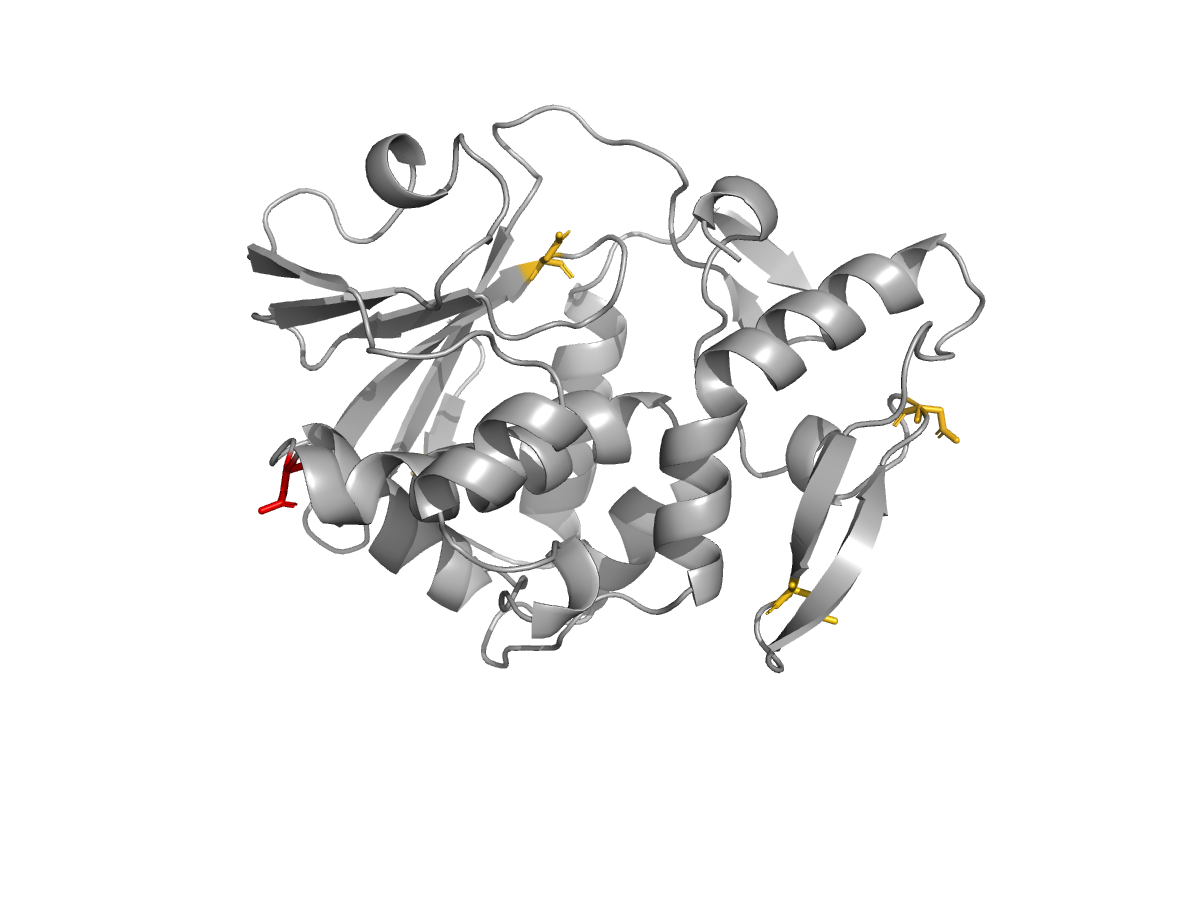
\includegraphics[width=\linewidth]{figures/feat170_RIP.png}
  \caption{\textbf{Feature 170} (AUROC 0.741)\\Cucurmosin (D0VWS7)\\Ribosome-inactivating protein}
\end{subfigure}\hfill
\begin{subfigure}[t]{0.245\linewidth}
  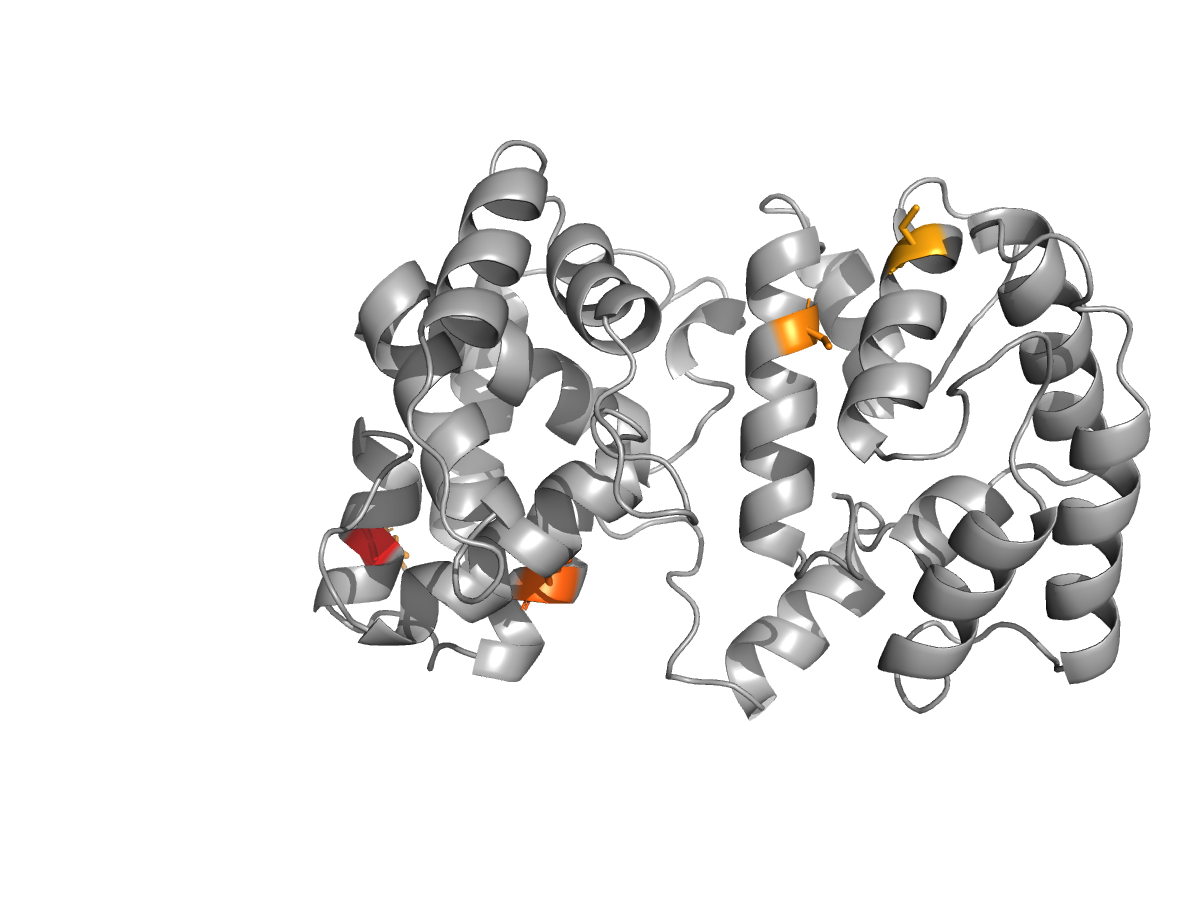
\includegraphics[width=\linewidth]{figures/feat351_mosquito.png}
  \caption{\textbf{Feature 351} (AUROC 0.731)\\D7L1 (A0A1S4K3K8)\\Mosquito salivary toxin}
\end{subfigure}
\caption{Top-firing residues for four leading RFD3 block-12 SAE features on partial-diffusion output structures. Red = highest activation, orange = moderate, gray = inactive. Feature 639's top-3 residues (99, 104, 109) cluster in a single alpha-helix of a viper neurotoxin. The other features fire on proteins from three other hazard classes, with similarly focal but less structurally concentrated activation.}
\label{fig:features}
\end{figure*}

\section{Background}

\paragraph{Sparse Autoencoders}
\label{sec:background}
Given an activation vector $x \in \mathbb{R}^{d}$, an SAE is an encoder
with a nonlinear activation function $\sigma$ and a linear decoder,
\begin{equation}
    z = \sigma(W_e x + b_e), \qquad \hat{x} = W_d z + b_d,
\end{equation}
trained to minimize a reconstruction loss, optionally with a sparsity penalty:
\begin{equation}
    \mathcal{L} = \mathbb{E}_x \big[\|x - \hat{x}\|_2^2\big] + \lambda \, \mathcal{S}(z).
\end{equation}
$W_e \in \mathbb{R}^{m \times d}$, $W_d \in \mathbb{R}^{d \times m}$ with $m \gg d$. Decoder columns are constrained to unit $L_2$ norm \cite{bricken2023monosemanticity}.

\paragraph{BatchTopK.} Rather than enforcing sparsity through an $L_1$ penalty on $z$, BatchTopK \cite{bussmann2024batchtopk} bakes it into the activation function: $\sigma$ keeps only the $BK$ largest pre-activations across an entire batch of $B$ samples,
\begin{equation}
    \sigma(u) = u \odot \mathbf{1}\!\big[u \geq \tau_{B,K}(U)\big],
\end{equation}
where $\tau_{B,K}(U)$ is the $(BK)$-th largest entry of the pre-activation tensor $U \in \mathbb{R}^{B \times m}$, yielding an average of $K$ active latents per sample. At inference, $\tau$ is replaced by a learned scalar threshold so that activations are batch-independent.

\paragraph{Matryoshka.} A Matryoshka SAE \cite{bussmann2025matryoshka} fixes a sequence of nested prefix sizes $m_1 < m_2 < \cdots < m_p = m$ and, for each prefix, decodes a reconstruction $\hat{x}^{(i)}$ using only the first $m_i$ latents (and the corresponding decoder columns). The total loss
\begin{equation}
    \mathcal{L}_{\text{matryoshka}} = \sum_{i=1}^{p} w_i \, \big\|x - \hat{x}^{(i)}\big\|_2^2
\end{equation}
forces earlier (smaller) prefixes to reconstruct $x$ on their own, encouraging them to capture coarse, general-purpose features, while later prefixes refine the reconstruction with finer-grained detail.

\subsection{Related Work}
\label{sec:related}

\paragraph{SAEs for protein models.}
\citet{simon2025interplm} recover thousands of biologically interpretable features from ESM-2 \cite{lin2023evolutionaryscale}; \citet{adams2025mechanistic} link ESM-2 SAE features to Gene Ontology (GO) terms and downstream properties; \citet{parsan2025interpretable} demonstrate causal steering of ESMFold's predicted surface area. FoldSAE \cite{zarzecki2025foldsae} trains SAEs on the token-level RFdiffusion \cite{watson2023rfdiffusion} and finds secondary-structure features. However, RFD3 operates on a mixed token-and-atom representation \cite{krishna2024rfaa,abramson2024alphafold3}.

\paragraph{Virulence prediction.}
Sequence-only classifiers have evolved from SVMs \cite{garg2008virulentpred} to PLM fine-tunes \cite{sun2024dtvf,chen2025virulenthunter}. The SOTA on the standard 576/576 benchmark is DTVF \cite{sun2024dtvf} at AUROC 0.92. None provide per-residue rationale.



\section{Methods}
\label{sec:methods}

\subsection{Models and activation collection}

RFD3 \cite{butcher2025rfdiffusion3} is an 18-block all-atom diffusion model; RF3 \cite{krishna2024rfaa} is its folding counterpart. Both operate on per-residue and per-atom representations. We attach PyTorch hooks to the diffusion transformer of each model and capture activations ($d = 768$) at three blocks in RFD3 (6, 8, 12) and two in RF3 (12, 16).

\subsection{Dataset}

We draw virulent sequences from SafeProtein \cite{fan2025safeprotein} and length-matched benign sequences from UniProt \cite{uniprot2023} (excluding toxin, virulence, and viral keywords; lengths 100--300\,aa), giving $n = 275$ pairs. For RF3 only we also use ToxinPred3 \cite{rathore2024toxinpred} ($n = 1200$); we exclude it from RFD3 evaluation because ToxinPred3 sequences lack PDB structures required for partial diffusion. For RFD3 inputs, we apply partial diffusion at $\partial t = 5$ (${\approx}5$\,\AA\ noise) to each sequence's PDB structure, simulating the activations the model produces when designing around that template. For RF3 we fold directly.




\subsection{SAE training}

For each (model, block) pair we train a Matryoshka BatchTopK SAE with dictionary size $m = 12{,}288$ ($16\times$ expansion), $K = 80$, five nested group fractions, learning rate $2.3 \times 10^{-4}$, and 20{,}000 steps on an L40 GPU, using the \texttt{dictionary\_learning} codebase \cite{marks2024dictionarylearning}. Training activations come from a held-aside corpus disjoint from SafeProtein. Trained SAEs explain $96.9\%$ of held-out activation variance ($L_0 = 79.9$, cossim $= 0.983$), with all features alive. Full hyperparameters are in \cref{app:hparams}.

\subsection{Virulence probes}

We mean-pool per-token SAE activations $z$ and raw activations $x$ over residues and denoising steps to obtain per-design vectors, then fit $L_2$-regularized logistic regression probes. We evaluate with 5-fold cross-validation under two regimes: \textit{random} (stratified) and \textit{homology-clustered}. Homology refers to shared evolutionary ancestry; without controlling for it, a probe can memorize fold-class identity from training homologs and appear to generalize when tested on related sequences. We cluster all sequences with mmseqs2 at 30\% identity \cite{steinegger2017mmseqs2} and assign whole clusters to folds. A length-only baseline yields AUROC $< 0.55$, ruling out a trivial length signal.

\subsection{Univariate feature scoring}

To identify individual SAE directions associated with virulence, we compute the univariate AUROC of each feature's mean activation against the class label. We then run Mann--Whitney U tests \cite{mann1947whitney} and apply Benjamini--Hochberg FDR correction \cite{benjamini1995controlling} to control for testing all 12{,}288 features simultaneously, reporting features with $q < 0.05$. Top features are visualized in PyMOL by mapping per-residue activations onto the diffusion output structure.



\begin{table}[tb]
  \caption{Held-out AUROC (mean $\pm$ std, 5 folds). \textbf{Cluster} = homology-clustered splits; \textbf{Random} = stratified random splits. \textbf{Bold} = best per dataset. Probe: \textit{raw} = raw activations; \textit{sae} = SAE-encoded features.}
  \label{tab:probes}
  \centering
  \begin{small}
    \begin{tabular}{llrccc}
      \toprule
      Model & Block & Probe & Cluster & Random \\
      \midrule
      \multicolumn{5}{l}{\textit{SafeProtein ($n$=275)}} \\
      \cmidrule(lr){1-5}
      \multirow{6}{*}{RFD3}
        & 6  & raw & $0.592 \pm 0.027$ & $0.722 \pm 0.073$ \\
        & 6  & sae & $0.599 \pm 0.106$ & $0.717 \pm 0.089$ \\
        & 8  & raw & $0.718 \pm 0.108$ & $0.785 \pm 0.052$ \\
        & 8  & sae & $0.699 \pm 0.136$ & $0.759 \pm 0.076$ \\
        & 12 & raw & $0.763 \pm 0.136$ & $0.863 \pm 0.063$ \\
        & 12 & sae & $\mathbf{0.817 \pm 0.102}$ & $\mathbf{0.877 \pm 0.025}$ \\
      \cmidrule(lr){1-5}
      \multirow{4}{*}{RF3}
        & 12 & raw & $0.738 \pm 0.095$ & $0.777 \pm 0.105$ \\
        & 12 & sae & $0.706 \pm 0.076$ & $0.771 \pm 0.075$ \\
        & 16 & raw & $\mathbf{0.776 \pm 0.098}$ & $\mathbf{0.776 \pm 0.058}$ \\
        & 16 & sae & $0.758 \pm 0.127$ & $0.774 \pm 0.088$ \\
      \midrule
      \multicolumn{5}{l}{\textit{ToxinPred3 ($n$=1200)}} \\
      \cmidrule(lr){1-5}
      \multirow{4}{*}{RF3}
        & 12 & raw & $0.807 \pm 0.069$ & $0.844 \pm 0.014$ \\
        & 12 & sae & $\mathbf{0.848 \pm 0.062}$ & $\mathbf{0.851 \pm 0.016}$ \\
        & 16 & raw & $0.803 \pm 0.061$ & $0.833 \pm 0.017$ \\
        & 16 & sae & $0.820 \pm 0.060$ & $0.835 \pm 0.021$ \\
      \bottomrule
    \end{tabular}
  \end{small}
  \vspace{-3ex}
\end{table}



\begin{figure}[tb]
\centering
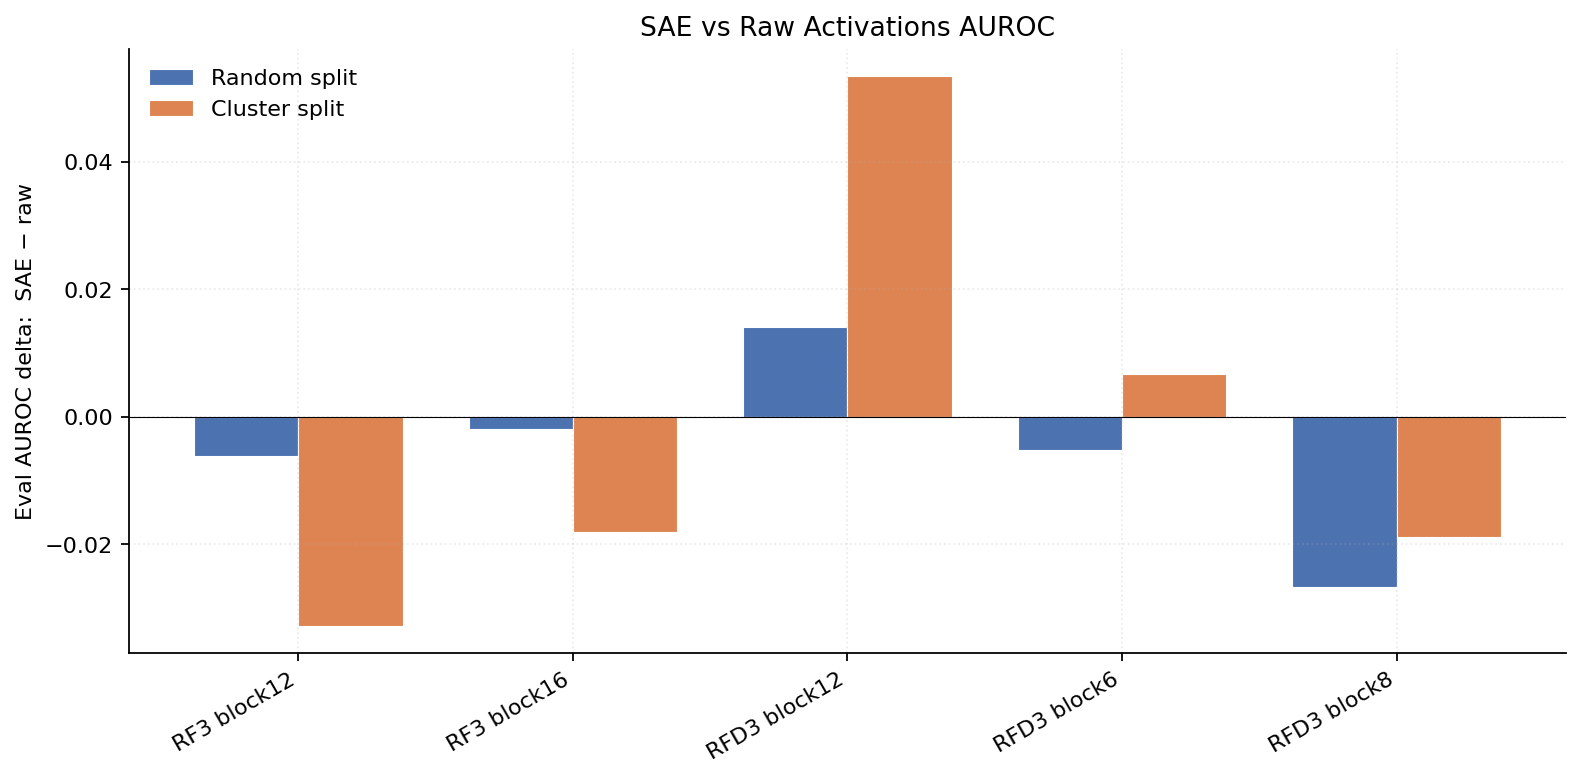
\includegraphics[width=\linewidth]{figures/03_sae_vs_raw_delta.png}
\caption{AUROC gap (SAE $-$ raw) per block and split. The only consistent positive spike is at RFD3 block 12, cluster split ($+0.054$).}
\label{fig:sae_vs_raw}
\vspace{-2ex}
\end{figure}


\begin{figure}[tb]
\centering
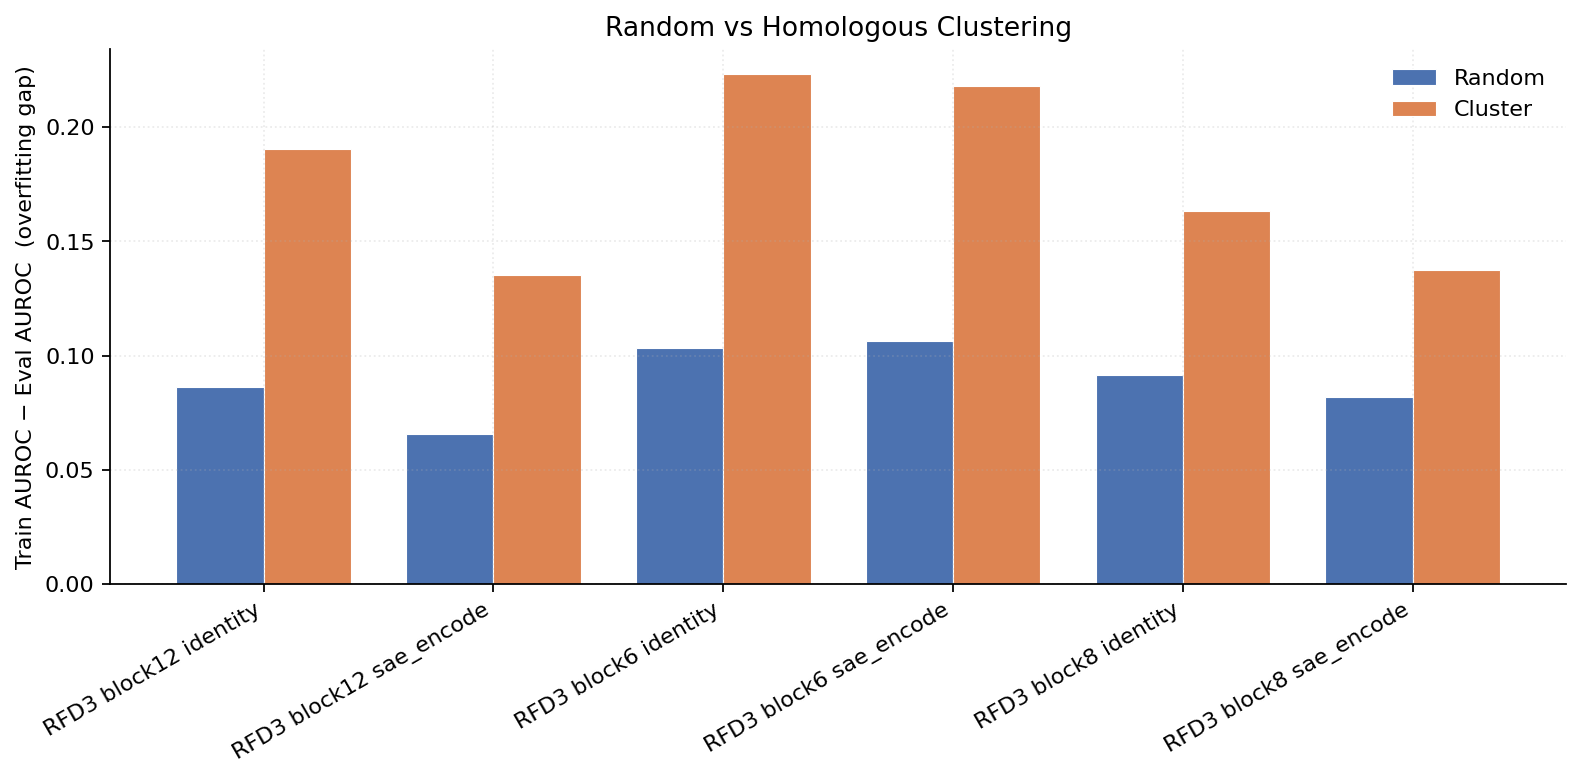
\includegraphics[width=\linewidth]{figures/02_train_vs_eval_gap.png}
\caption{Random$-$homology AUROC gap. Larger = more family memorization. Block 6 peaks; block-12 SAE is smallest.}
\vspace{-2ex}
\label{fig:gap}
\end{figure}


\begin{figure*}[tb]
\centering
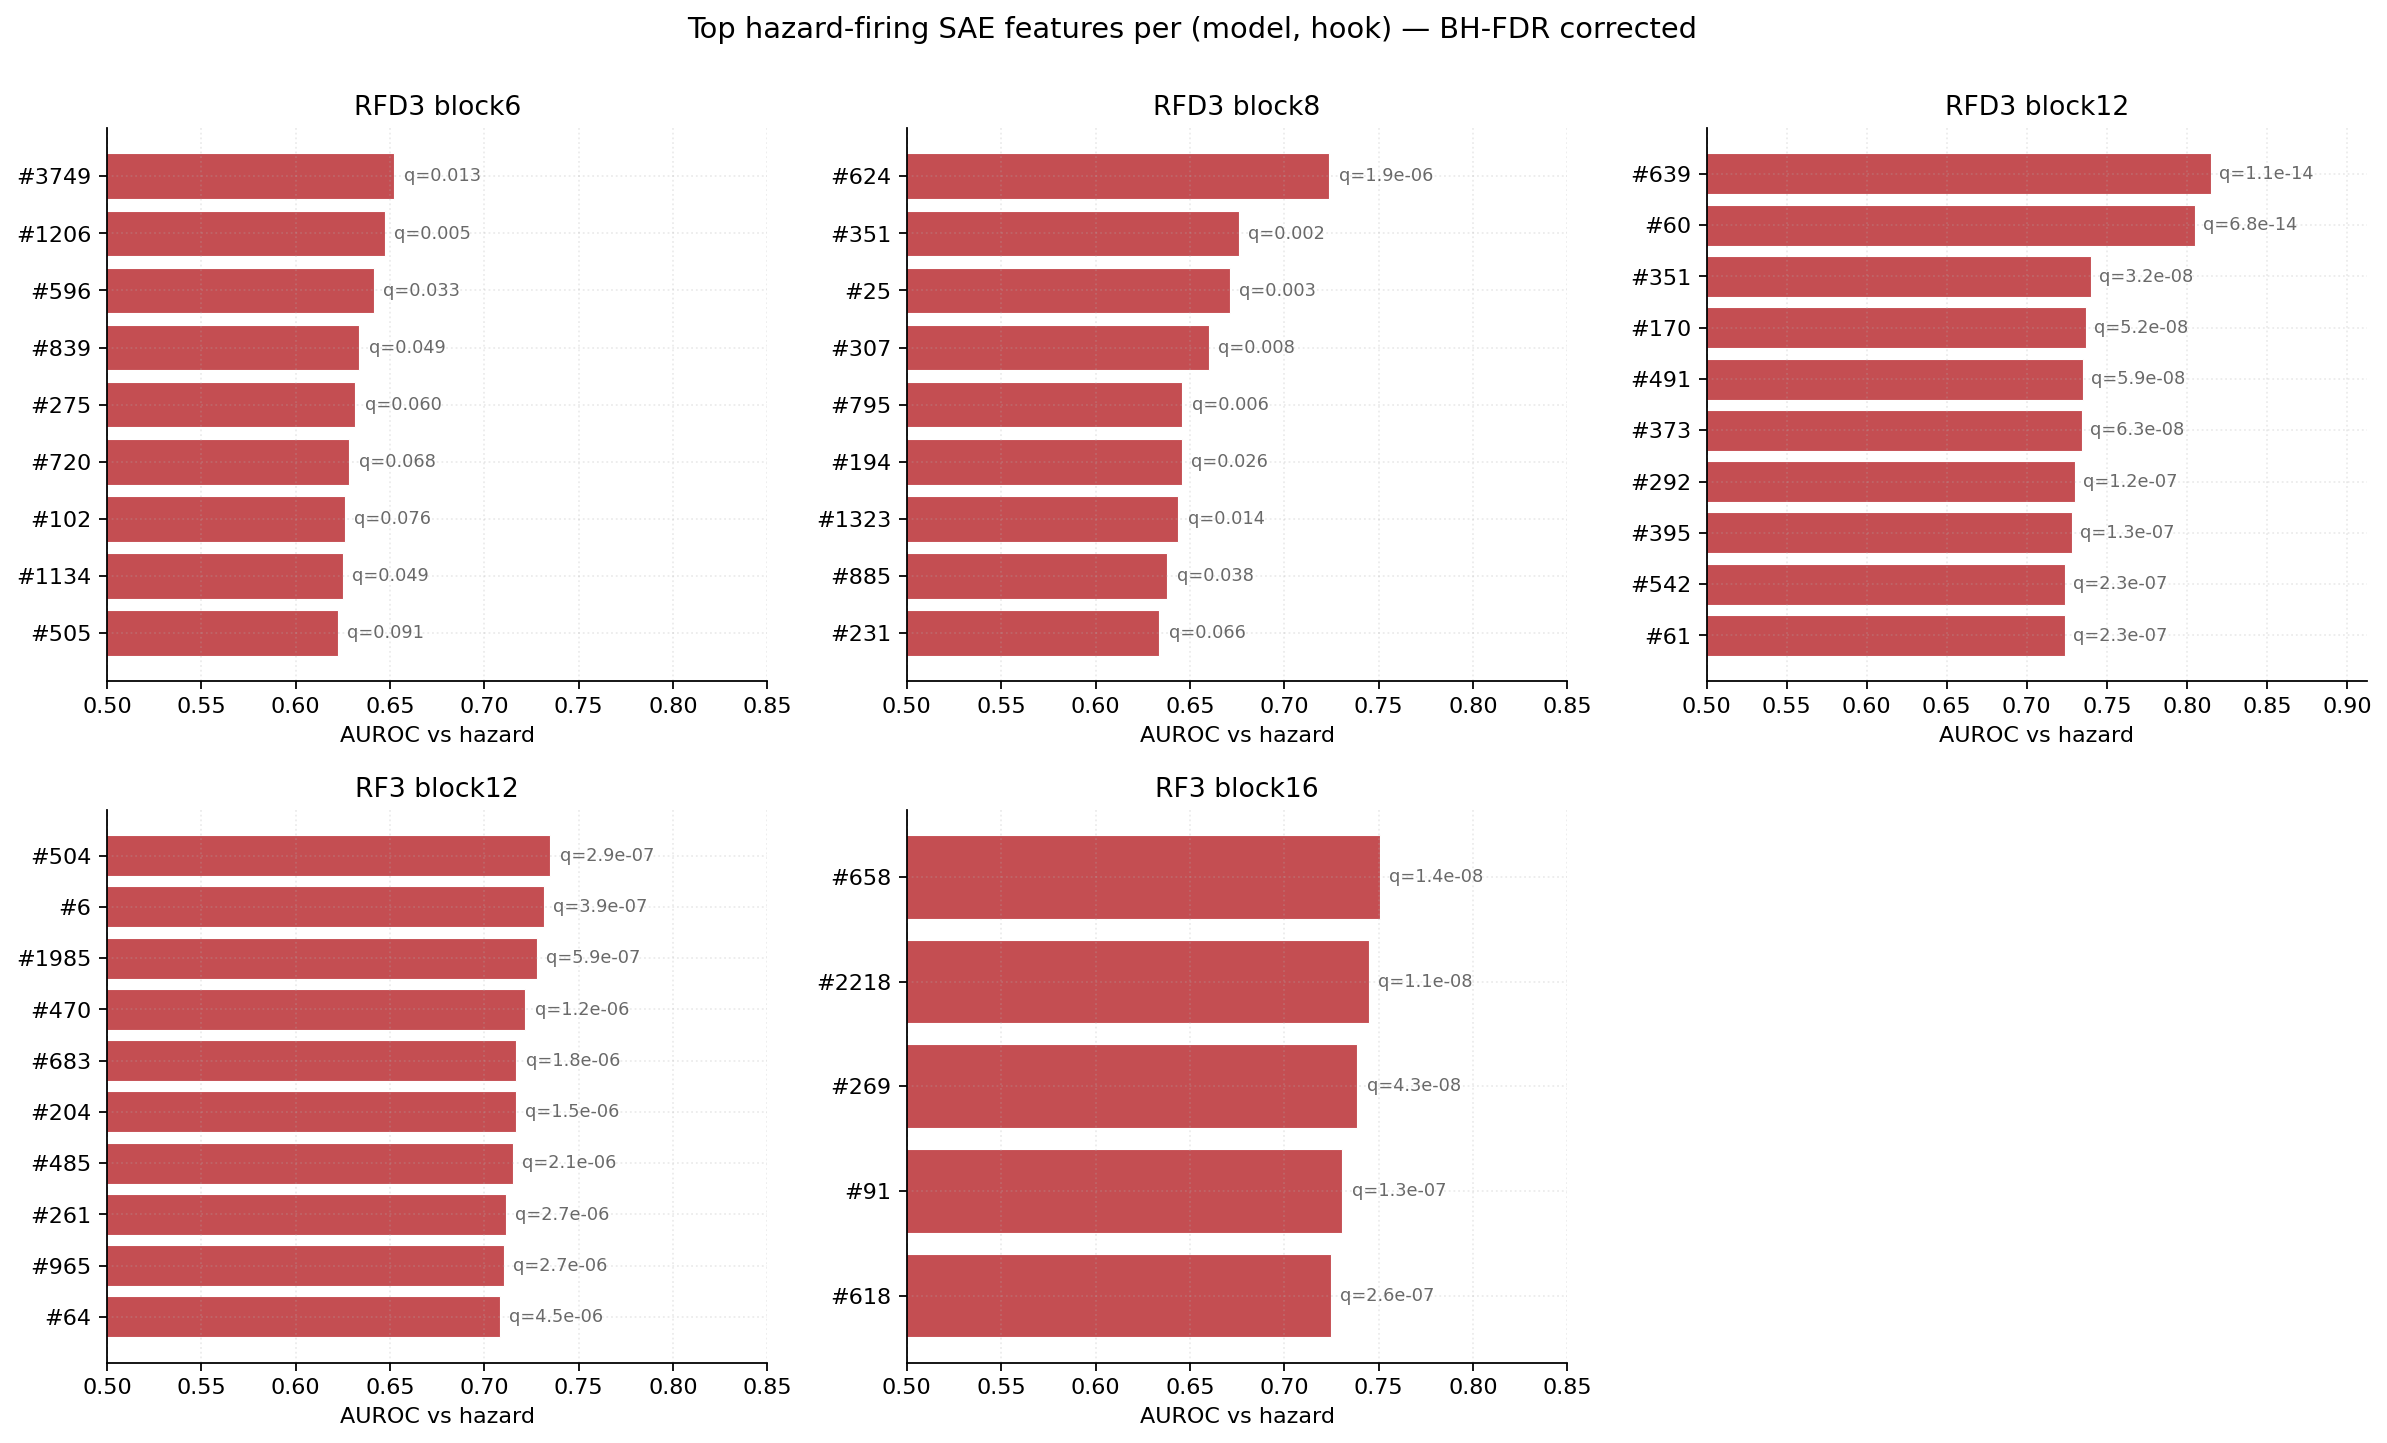
\includegraphics[width=0.95\linewidth]{figures/04_top_hazard_features.png}
\vspace{-1ex}
\caption{Top-10 hazard-firing SAE features per (model, block), ranked by univariate AUROC with BH-corrected $q$-values. Feature quality (peak AUROC and number of discoveries) grows with depth in RFD3, with block-12 features reaching AUROC ${\geq}0.80$.}
\label{fig:top_features}
\vspace{-2ex}
\end{figure*} 



\section{Results}
\label{sec:results}

\Cref{tab:probes} reports held-out AUROC across all conditions. The best overall probe is RFD3 block-12 SAE features: AUROC $0.877 \pm 0.025$ random, $0.817 \pm 0.10$ clustered. Performance grows with depth in RFD3 (block 6 clustered: $0.592$; block 12 clustered: $0.817$) but is flat across RF3 blocks.


\subsection{SAE features beat raw activations at block 12}

\Cref{fig:sae_vs_raw} shows the AUROC delta (SAE minus raw) per block. The SAE adds $+0.054$ at RFD3 block 12 under cluster splits and is neutral or negative everywhere else. For RF3 / ToxinPred3 the SAE also adds $+0.041$ at block 12 under cluster splits. We attribute the block-12 gain to polysemanticity: by that depth the residual stream mixes many structural concepts, and dictionary learning untangles them into directions that a low-capacity probe can use. Earlier blocks are already sufficiently aligned that the SAE projection is unnecessary.


The features fire on proteins from distinct hazard classes: a viper presynaptic neurotoxin, a monkeypox immune-evasion phosphatase, a plant ribosome-inactivating protein, and a mosquito salivary toxin (See \Cref{fig:features}). Activations are localized, with each feature highlighting a handful of residues per structure. Feature 639 is the most spatially coherent, with its top three residues (99, 104, 109) all falling within a single annotated alpha-helix (positions 96--114) of ammodytoxin A. This pattern reproduces across independent partial-diffusion runs (\cref{app:moreviz}).

\subsection{Homology memorization audit}

The random-homology AUROC gap (\cref{fig:gap}) is largest at RFD3 block 6 ($0.22$ cluster), consistent with early denoising blocks collapsing toward fold-family templates. The block-12 SAE has the smallest gap ($0.13$), suggesting this is where class-discriminative, family-generalizable structure lives.


\subsection{Individual hazard features}

After BH correction, significant features ($q < 0.05$) grow from ${\sim}70$ at RFD3 block 6 to ${\sim}340$ at block 12, where the top feature reaches AUROC $0.819$ ($q \approx 10^{-13}$). \Cref{fig:top_features} shows the top-10 features per (model, block) ranked by univariate AUROC, illustrating both the depth trend and the range of per-feature discrimination. \Cref{fig:features} maps activations for the four leading features onto diffusion output structures.

\subsection{Comparison with sequence-only classifiers}

Our best probe (RFD3 block-12 SAE, random, $0.877$) is competitive with sequence-only specialists: VF-Pred \cite{singh2024vfpred} ($0.84$), VirulentPred \cite{garg2008virulentpred} ($0.86$), and DTVF \cite{sun2024dtvf} ($0.92$). This is not a fair head-to-head comparison: we train a simple logistic probe rather than a task-specific classifier, and our dataset ($n = 275$) differs from the standard benchmark. The point is that model-internal probing can approach specialist accuracy while also localizing the signal to individual residues.

\section{Discussion}
\label{sec:discussion}

\paragraph{Block selection.}
\citet{gao2025scaling} and \citet{templeton2024scaling} report that SAE feature quality peaks at middle-to-late transformer layers; block 12 of 18 in RFD3 is the analogous position. All three of our block-12 metrics converge: largest SAE-over-raw gain (\cref{fig:sae_vs_raw}), smallest memorization gap (\cref{fig:gap}), and most significant features. RFD3's earlier blocks underperform under homology-clustering while RF3's do not, consistent with the denoising process encoding fold-family identity at early timesteps.

\paragraph{Limitations.}
The dataset is small ($n = 275$, ${\sim}55$ per fold), so confidence intervals are wide. Hookpoint selection followed LLM practice rather than a principled ablation. Mean-pooling discards spatial information that a per-residue probe could use. Preliminary activation-steering experiments showed no effect on DTVF-scored outputs (\cref{app:steering}); steering in the partial-diffusion setting remains an open problem.

\section{Conclusion}

We showed that an SAE trained on RFdiffusion3's block-12 residual stream improves virulence probe AUROC over raw activations ($+0.054$ under homology-clustered splits), and that individual SAE features fire selectively on hazardous structures with per-residue localization. This opens a path to runtime monitoring and interpretable audit of generative protein design models.


\bibliography{example_paper}
\bibliographystyle{icml2026}

\appendix
\onecolumn

\section{SAE Training Hyperparameters}
\label{app:hparams}

\begin{table}[h]
\centering
\begin{tabular}{ll}
\toprule
Activation dim $d$ & 768 \\
Dictionary size $m$ & 12{,}288 ($16\times$) \\
Top-K & 80 \\
Group fractions & $(0.0625, 0.125, 0.1875, 0.25, 0.375)$ \\
aux-K alpha & $0.03125$ \\
Learning rate & $2.3 \times 10^{-4}$ \\
Warmup / total steps & $1000$ / $20{,}000$ \\
Batch size & $4096$ \\
Hardware & 1 $\times$ L40 (48\,GB) \\
\bottomrule
\end{tabular}
\caption{SAE training hyperparameters (all (model, block) pairs identical).}
\end{table}

\section{Per-Fold Probe Results}
\label{app:perfold}

\begin{table}[h]
\centering
\begin{tabular}{lcc}
\toprule
Fold & N(eval) & AUROC \\
\midrule
0 & 59 & 0.982 \\
1 & 54 & 0.770 \\
2 & 54 & 0.777 \\
3 & 54 & 0.717 \\
4 & 54 & 0.838 \\
\midrule
Mean $\pm$ std & --- & $0.817 \pm 0.102$ \\
\bottomrule
\end{tabular}
\caption{Per-fold AUROC, RFD3 block 12, SAE, homology-clustered splits.}
\label{tab:perfold_block12}
\end{table}

\section{Additional Feature Visualizations}
\label{app:moreviz}

\begin{figure}[h]
\centering
\begin{subfigure}[t]{0.31\linewidth}
  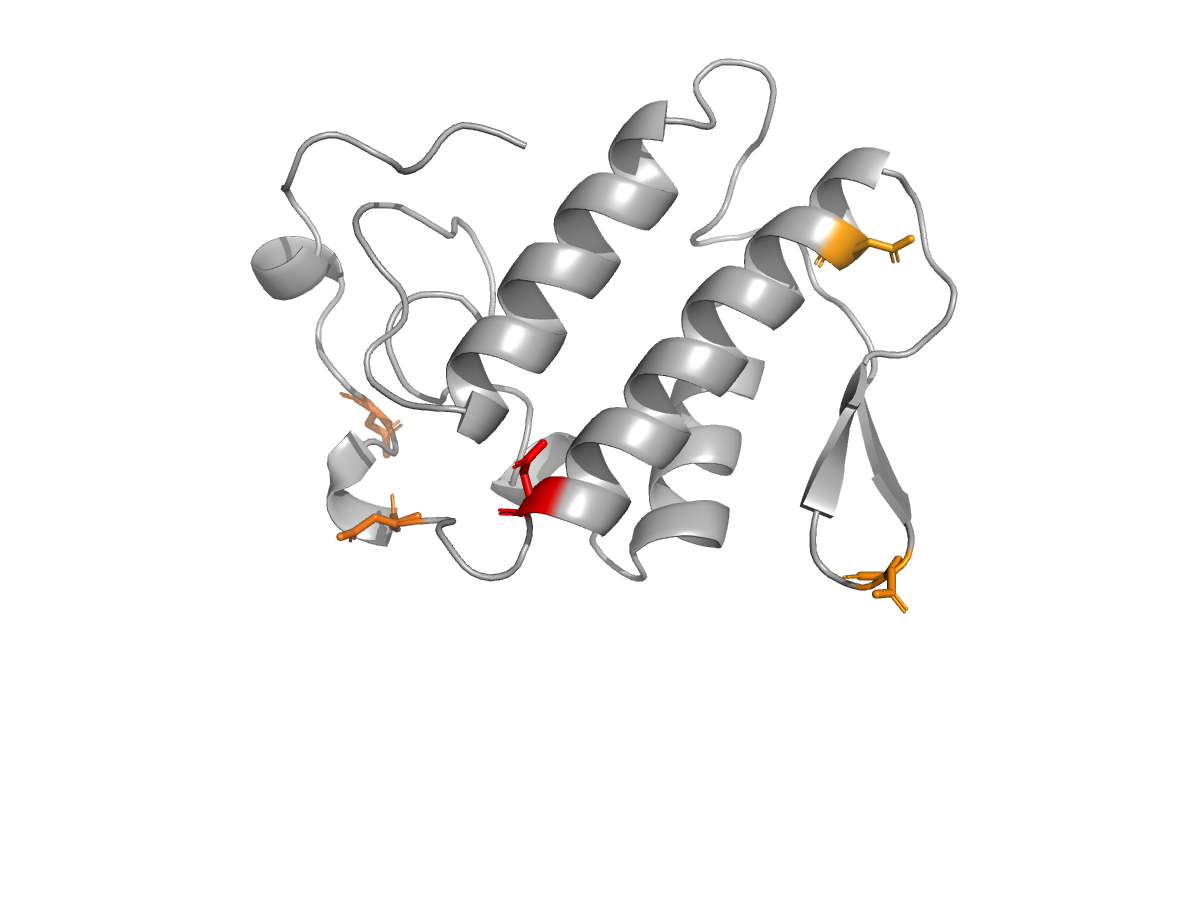
\includegraphics[width=\linewidth]{figures/feat639_P00626_m1.png}
  \caption{Feature 639, ammodytoxin A, run 2. Residues 99, 104, 109 highlighted again.}
\end{subfigure}\hfill
\begin{subfigure}[t]{0.31\linewidth}
  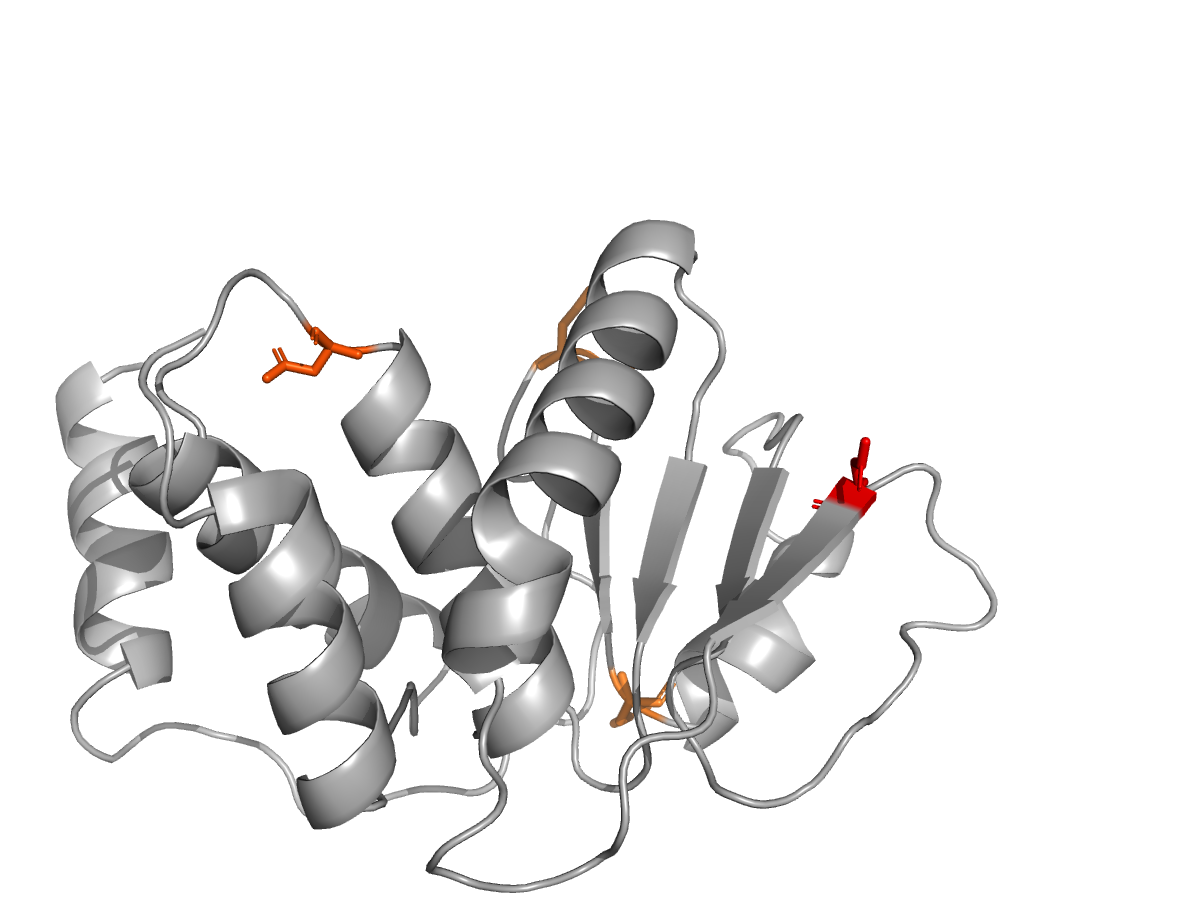
\includegraphics[width=\linewidth]{figures/feat060_MPXV_m1.png}
  \caption{Feature 60, MPXV OPG106, run 2.}
\end{subfigure}\hfill
\begin{subfigure}[t]{0.31\linewidth}
  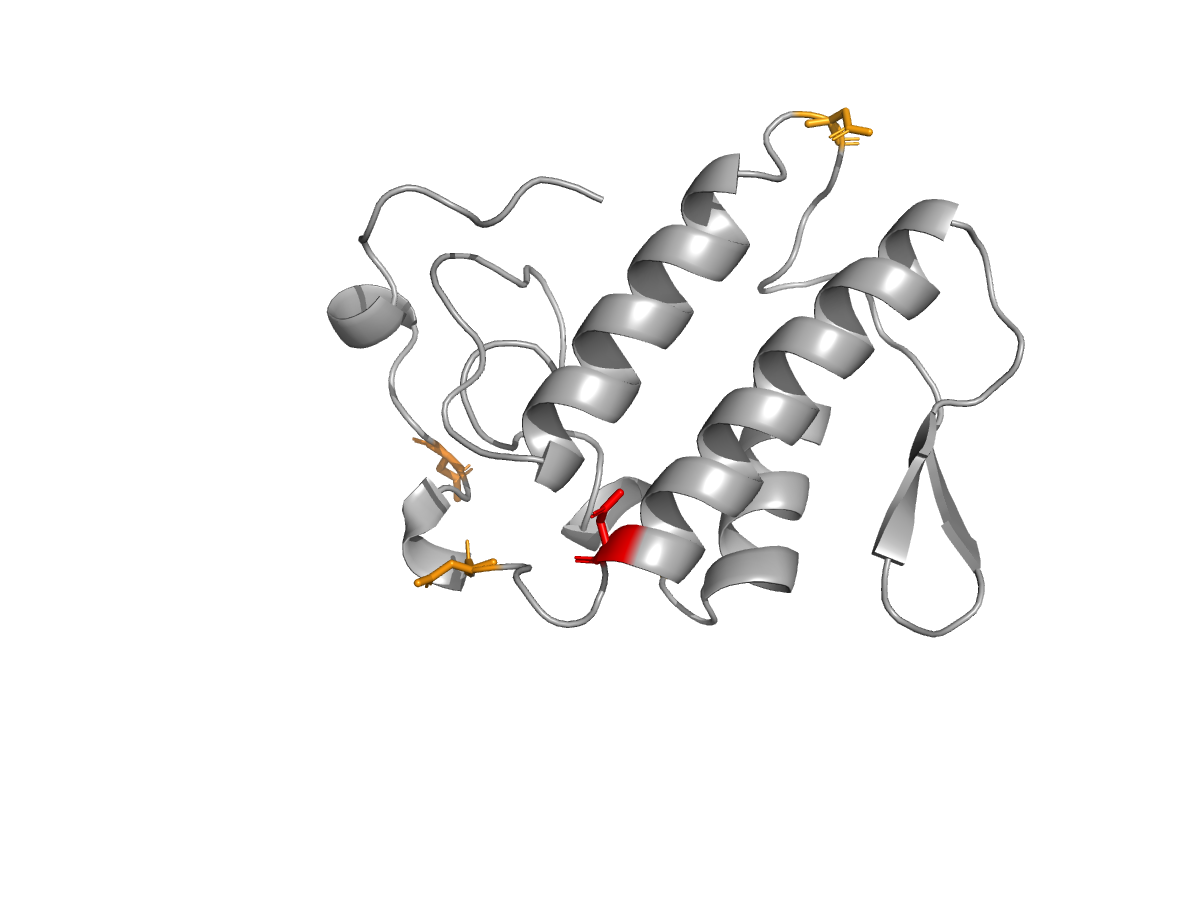
\includegraphics[width=\linewidth]{figures/feat491_P00626.png}
  \caption{Feature 491 (AUROC 0.743), ammodytoxin A. Different residues from those of feature 639, suggesting distinct structural determinants.}
\end{subfigure}
\caption{Reproducibility check and additional features. Same color scale as \cref{fig:features}.}
\label{fig:feat_extra}
\end{figure}

\section{Negative Result: Steering}
\label{app:steering}

We added a diff-of-means hazard direction (block 12, $\alpha \in \{1,2,4,8\}$) during partial-diffusion redesign of 10 hazardous PDB inputs at $\partial t \in \{5, 50\}$, then scored the designed sequences with DTVF \cite{sun2024dtvf}. DTVF probabilities were constant across $\alpha$, suggesting either the partial-diffusion setting does not provide enough denoising steps for the perturbation to propagate, or sequence extraction dominates the structural steering. We report this as a baseline for future work.

\end{document}
